\chapter{Results of experiments with \carrp}
\label{app:cap}
\textit{This Appendix presents graphically a summary of individuals runs using \carrp. Figures show a \textit{box-plot} representation for different strategies and a bar representation for the percentage of winner solvers types.}

\vspace{2ex}\vfill
\minitoc
\newpage

\section{Comparison between sequential and parallel runs}

%\begin{wrapfigure}{R}{0.4\textwidth}
%\centering
%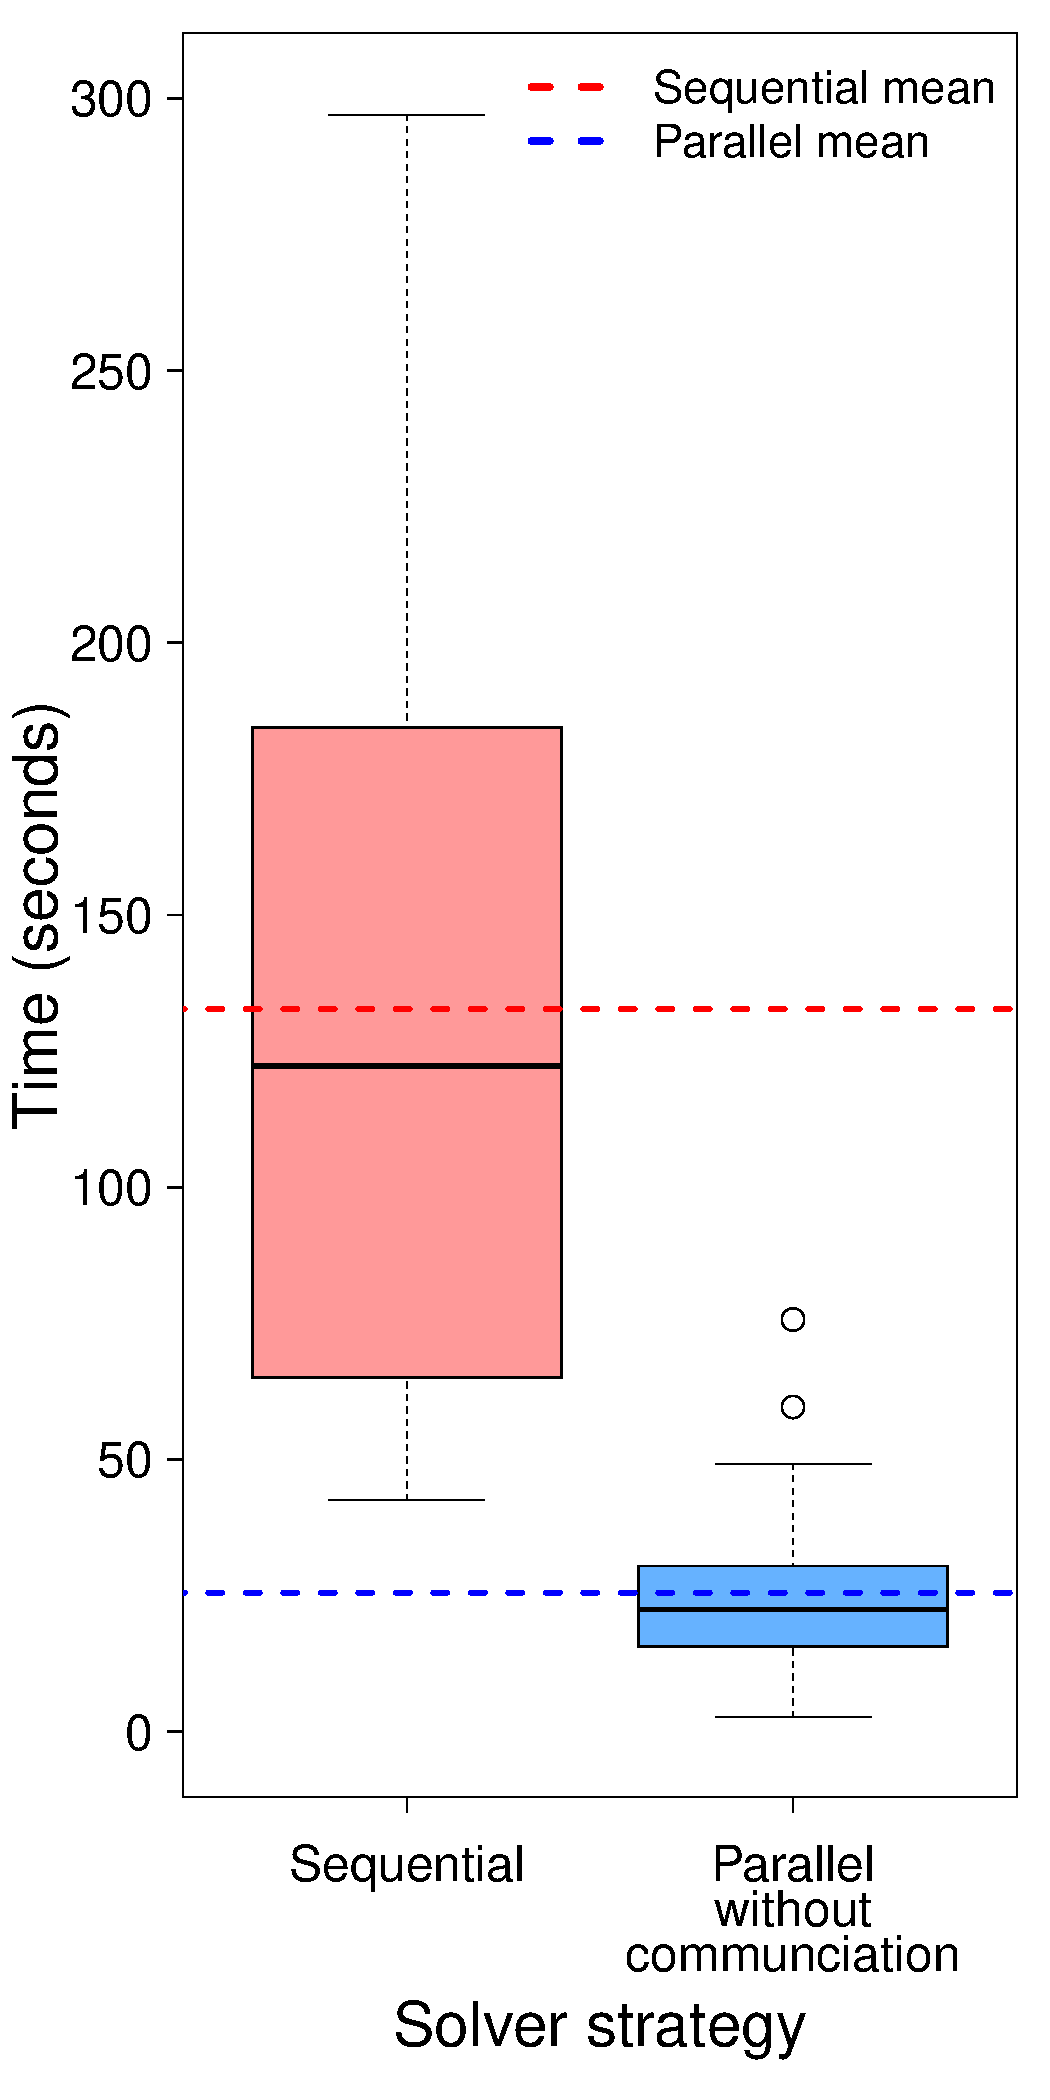
\includegraphics[width=0.3\textwidth]{c19_select_BP.pdf}
%\caption{Comparison between sequential and parallel runs to solve \CARRP{} 19 using \posl}\label{boxplot:19}
%\end{wrapfigure}
%
%Figure~\ref{boxplot:19} shows that the approach in parallel largely outperforms the sequential one. this is because this problem is very sensitive to the starting point. In the graph we can observe that all parallel runs are far below the mean of sequential runs. In addition, the minimum sequential runtime is higher that the 50\% of the parallel runs.

\begin{minipage}[c]{0.50\textwidth}
Figure~\ref{boxplot:19} shows that the approach in parallel largely outperforms the sequential one. this is because this problem is very sensitive to the starting point. In the graph we can observe that all parallel runs are far below the mean of sequential runs. In addition, the minimum sequential runtime is higher that the 50\% of the parallel runs.
\end{minipage}\hspace{0.05\textwidth}
\begin{minipage}[c]{0.40\textwidth}
\centering
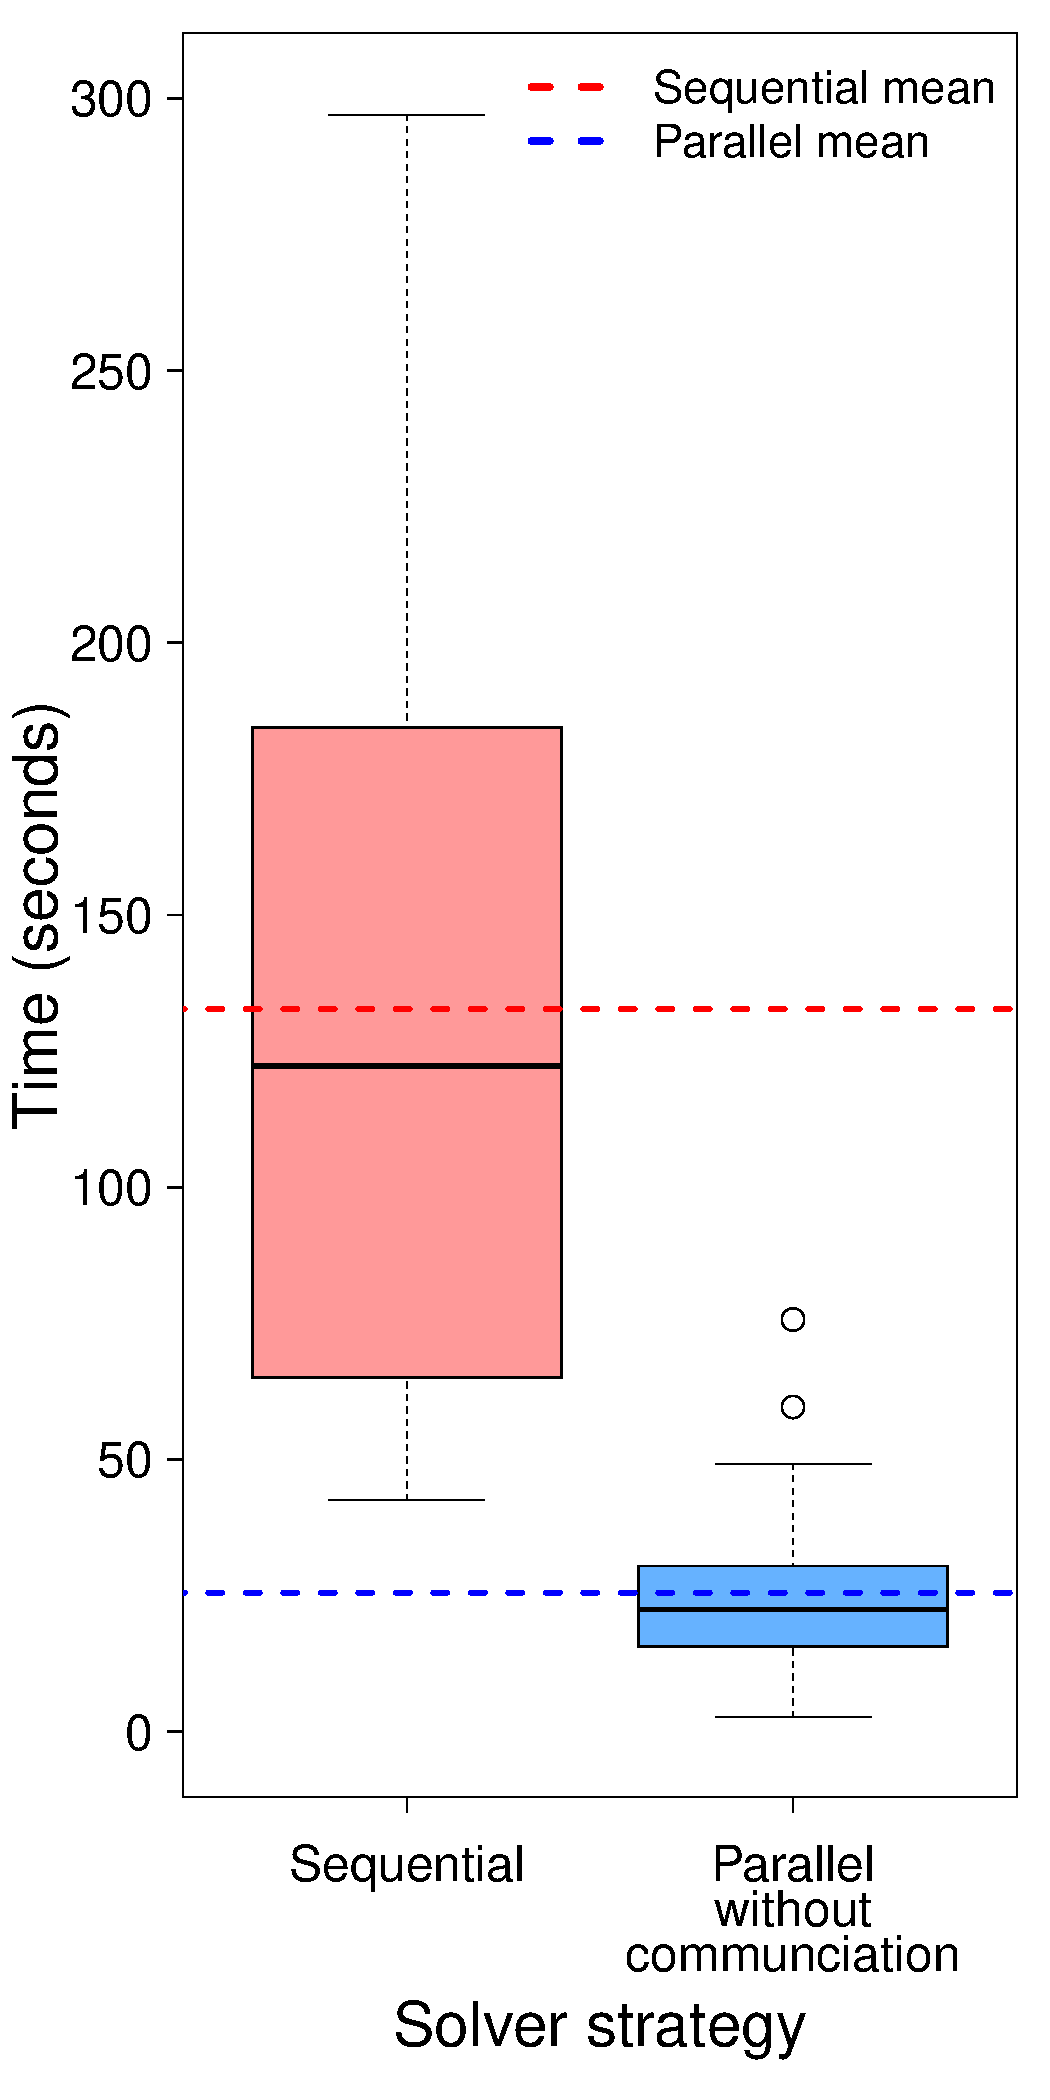
\includegraphics[width=0.8\textwidth]{c19_select_BP.pdf}
\captionof{figure}{Comparison between sequential and parallel runs to solve \CARRP{} 19 using \posl}\label{boxplot:19}
\end{minipage}

\section{Comparison between \commstrs}

In Figure~\ref{boxplot:comm}, labels of the x-axis correspond to the following strategies:

\poslcaptiondesciption{
\begin{tabular}[t]{rl}
\textbf{NC}: & Non communication strategy \\
\textbf{A1-1}: & 100\% of communicating solvers performing the \commstr{} A \oneTone \\
\textbf{B1-1}: & 100\% of communicating solvers performing the \commstr{} B \oneTone \\
\textbf{A1-n}: & 100\% of communicating solvers performing the \commstr{} A \oneTn \\
\textbf{B1-n}: & 100\% of communicating solvers performing the \commstr{} B \oneTn \\
\textbf{50A1-1}: & 50\% of communicating solvers performing the \commstr{} A \oneTone \\ 
\textbf{50B1-1}: & 50\% of communicating solvers performing the \commstr{} B \oneTone \\
\textbf{50A1-n}: & 50\% of communicating solvers performing the \commstr{} A \oneTn \\
\textbf{50B1-n}: & 50\% of communicating solvers performing the \commstr{} B \oneTn \\
\end{tabular}
}

Figure~\ref{boxplot:comm} shows that \commstrs{} of type \texttt{A} provide better and more stable results: the lower quartile value of parallel runs (\texttt{NC}) is higher that the upper quartile value of both \commstrs{} (\texttt{A1-1} an \texttt{A1-n})

\begin{figure}[h]
\centering
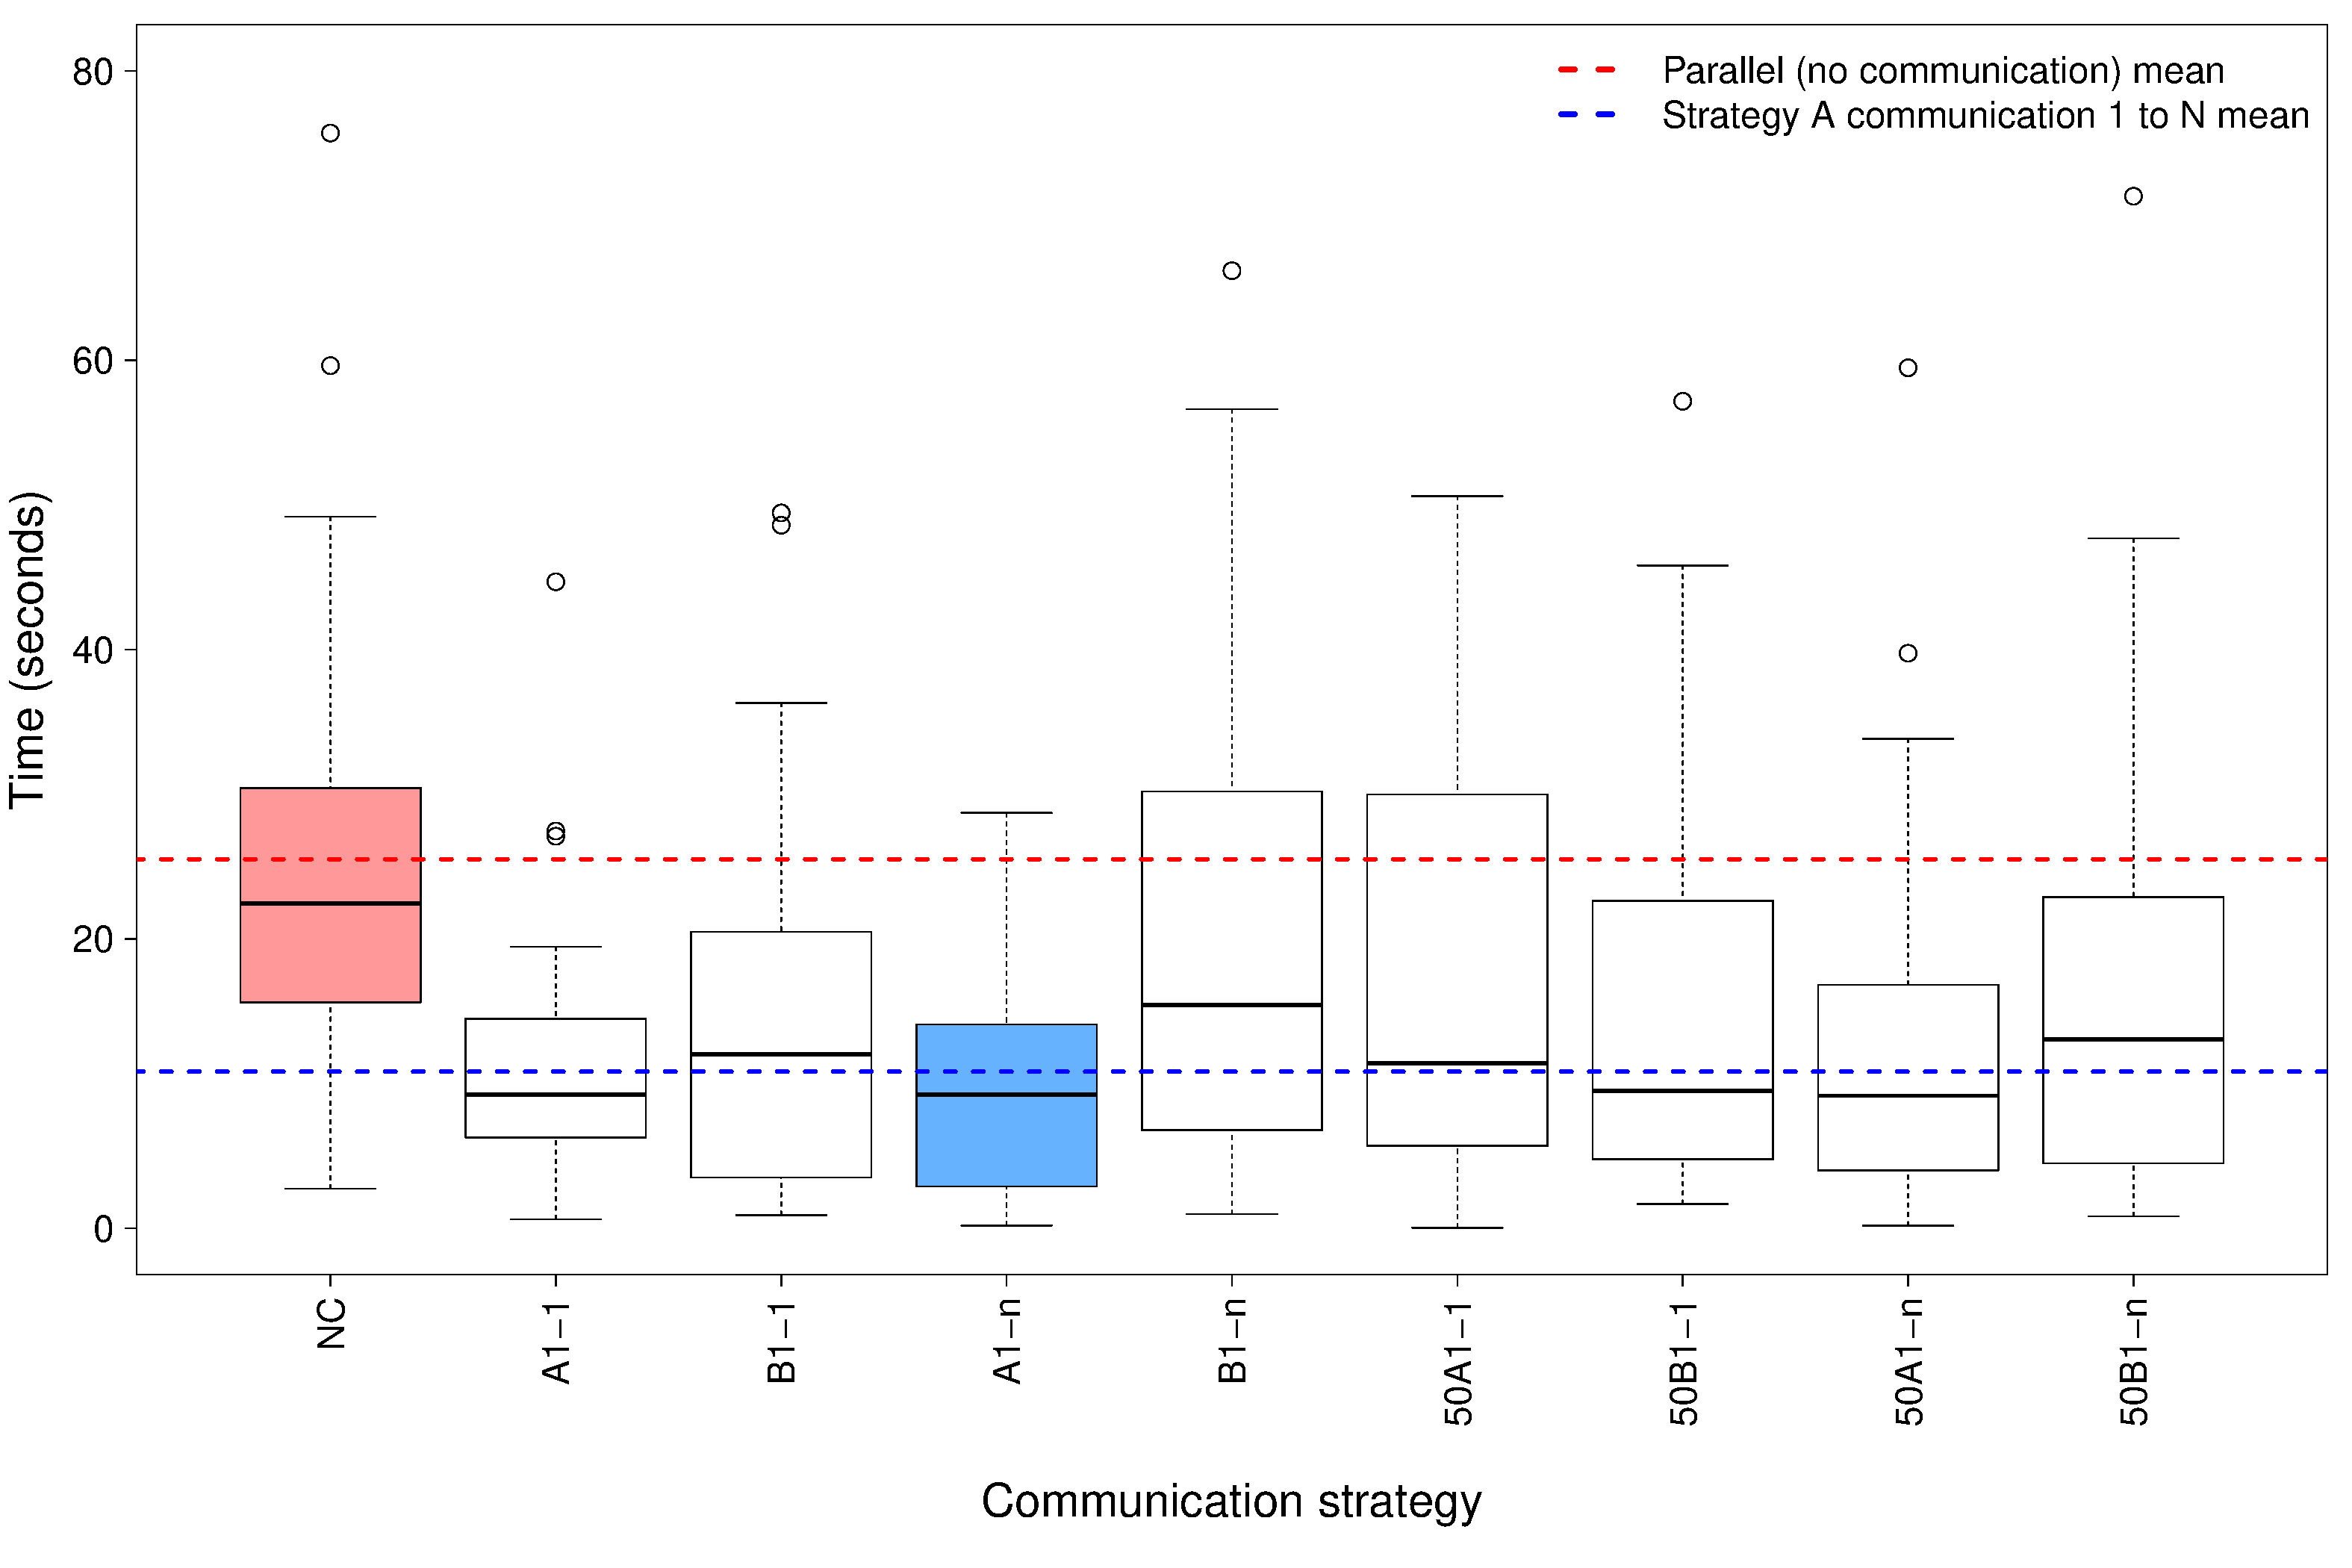
\includegraphics[width=0.8\textwidth]{c19_comm_BP.pdf}
\caption{Different communication strategies to solve \CARRP{} 19 using \posl}\label{boxplot:comm}
\end{figure} 



\section{Winner solver type representation}

Figure~\ref{barplot:19} represents the percentage of winner solvers for each communication strategy, according to three different types:

\poslcaptiondesciption{
\begin{tabular}[t]{rl}
\receiver{Receiver}: & Receiver solver wining thanks to the received information \\
\sender{Sender}: & Sender solver \\
%\nonreceiver{Pasive receiver}: & Receiver solver wining without using the received information \\
\nocomm{Non communicating}: & Non communicating solver \\
\end{tabular}
}

The bars graph in Figure~\ref{barplot:19} is self-explained: percentages of winner communicating solvers match with percentage of communicating solvers participating in the respective \commstr.

\begin{figure}[!h]
\centering
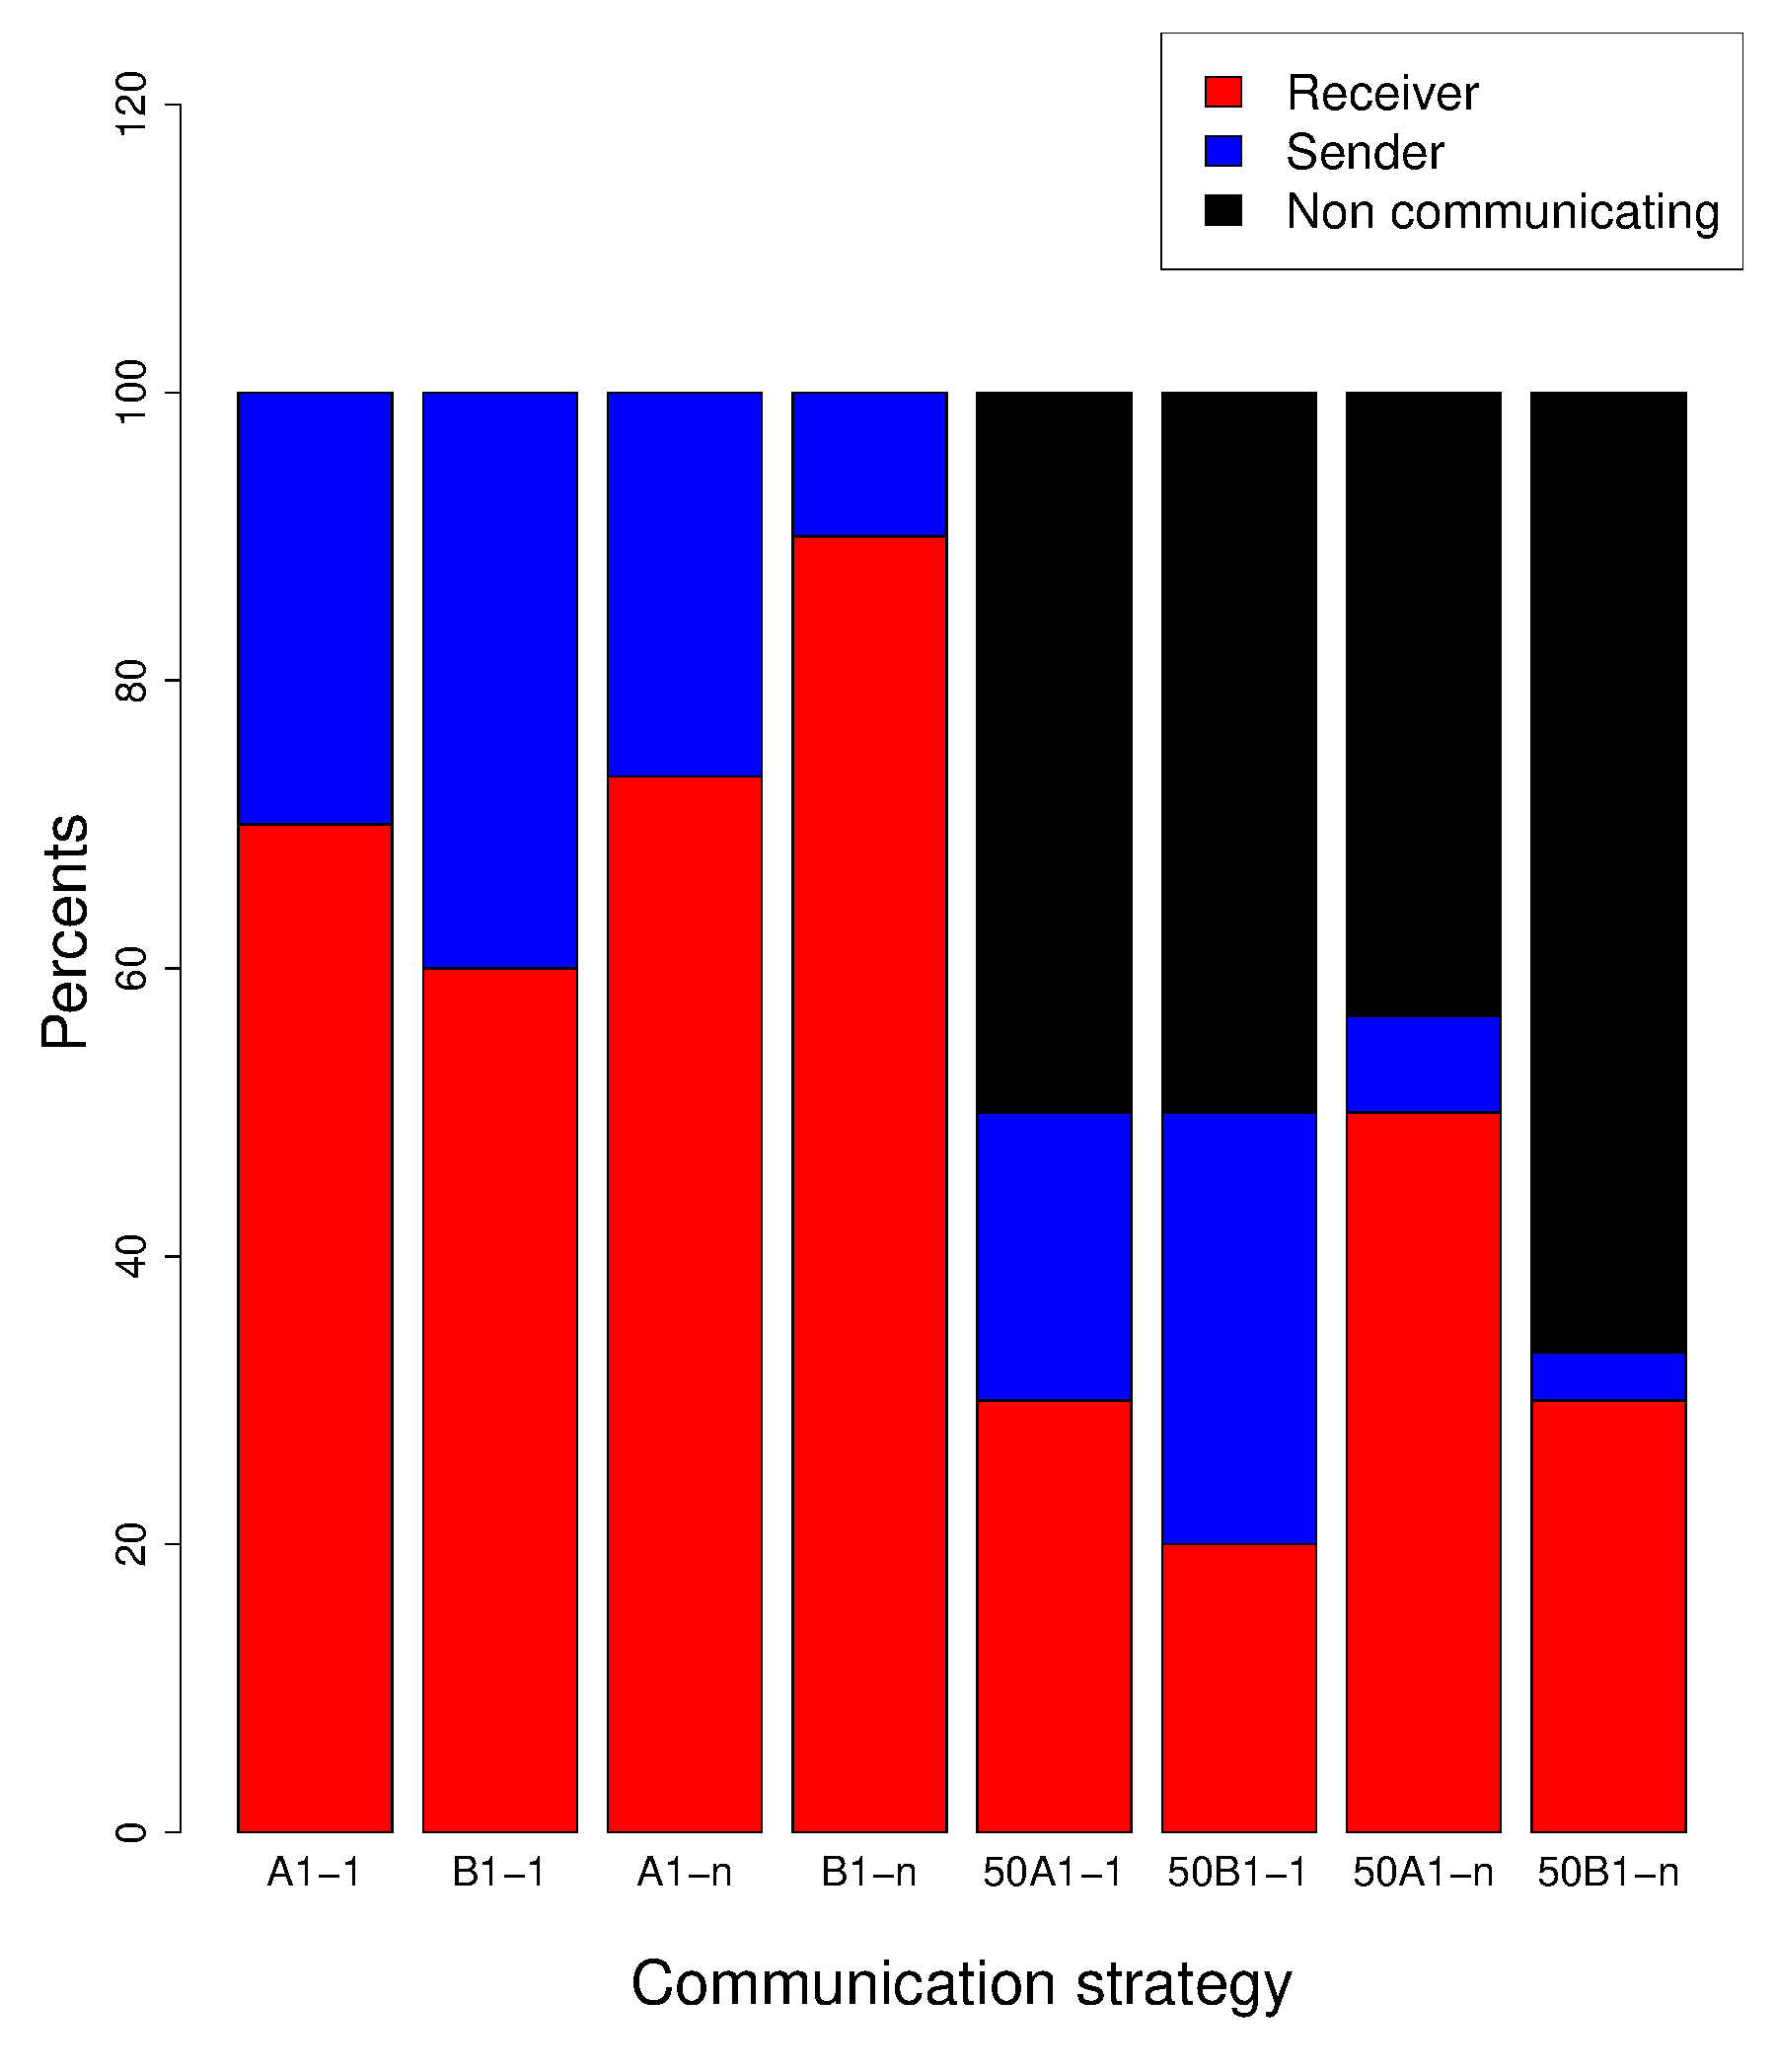
\includegraphics[width=0.6\textwidth]{c19_per_BP.pdf}
\caption{Solver proportion for each communication strategy to solve \CARRP{} 19 using \posl}\label{barplot:19}
\end{figure}